\newgeometry{top=1cm, bottom=2cm}
\section{Vektorräume}
\begin{figure}[h!]
    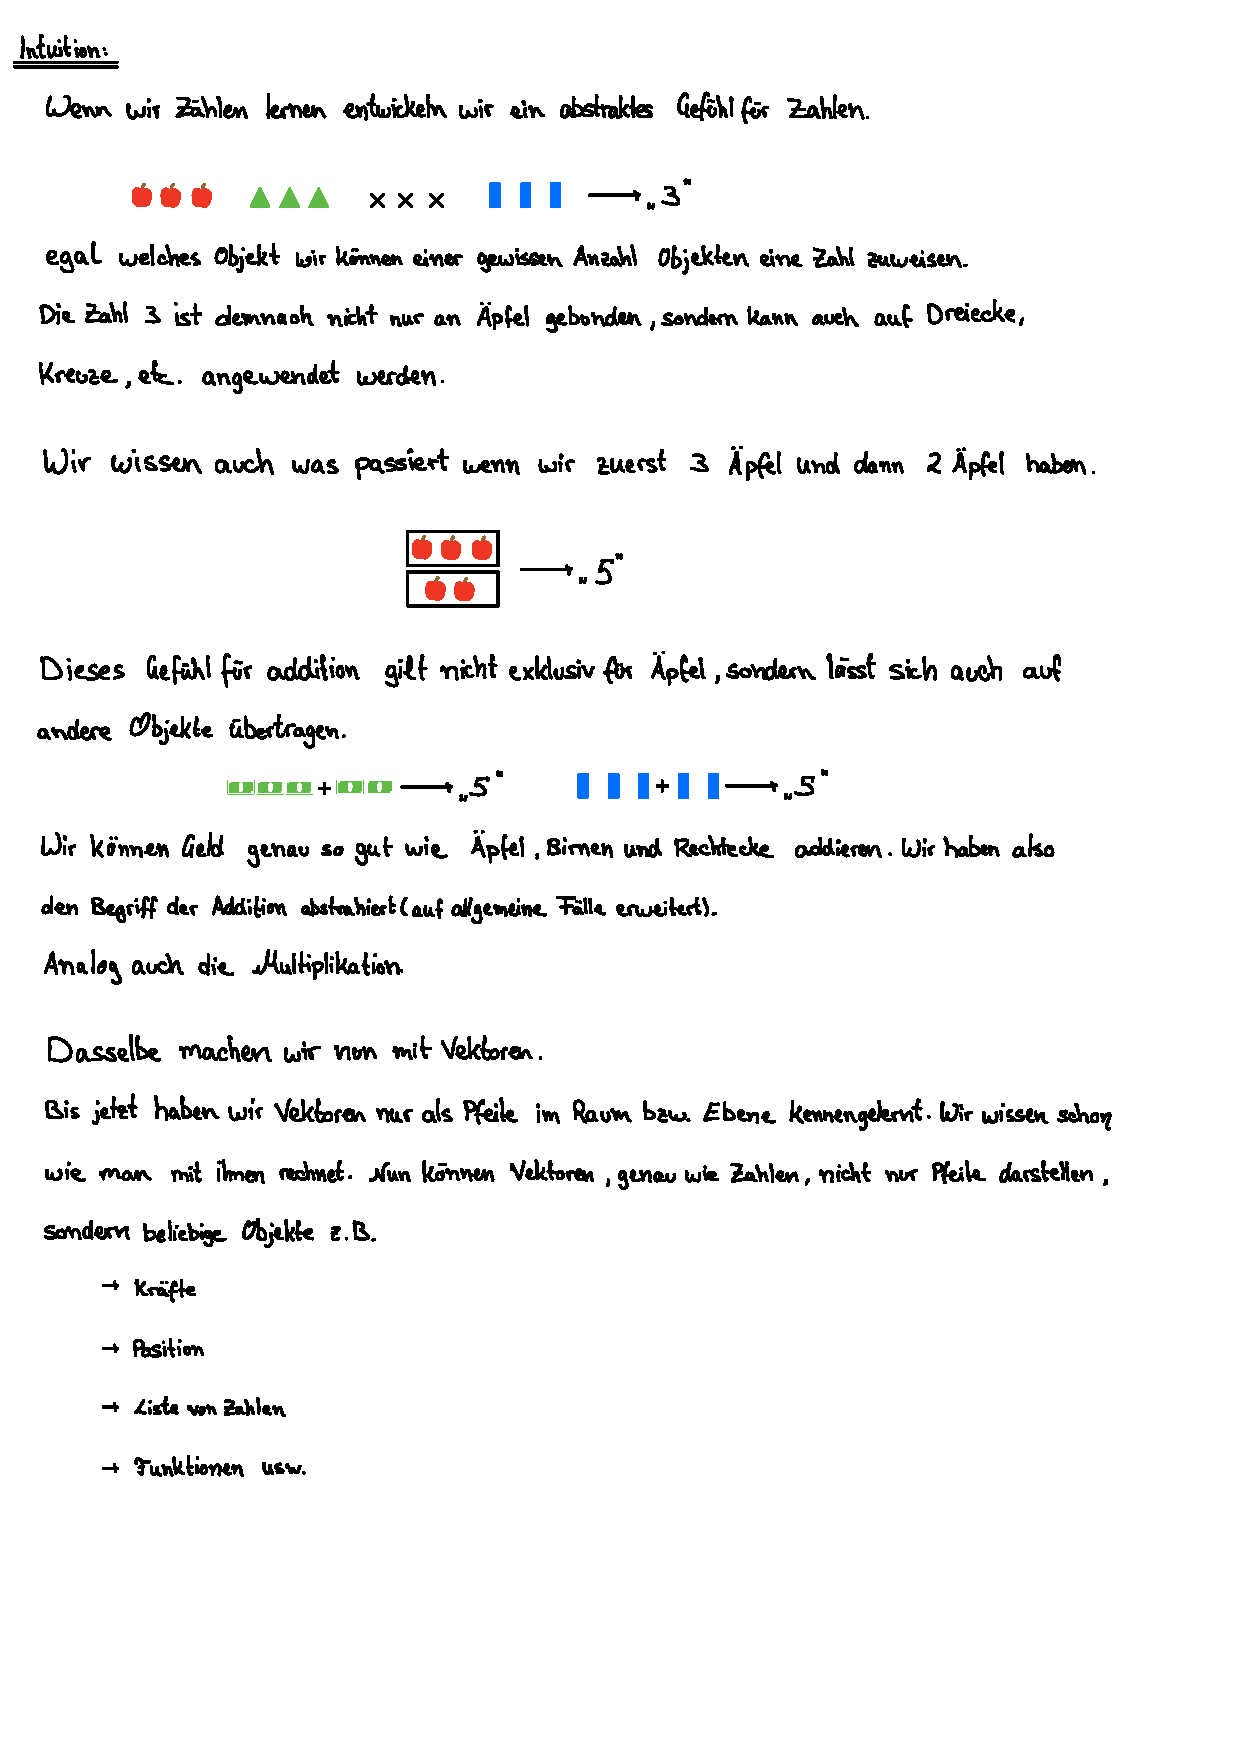
\includegraphics[page=1, scale=0.842]{pdf/04_Vektorraeume.pdf}
\end{figure}
\newpage
\includepdf[pages={2-}, 
            pagecommand={\thispagestyle{plain}}, 
            scale=0.95]{pdf/04_Vektorraeume.pdf}

\newgeometry{top=2.5cm, bottom=2cm}

\subsection{Beispielaufgaben} 

\vspace{1cm}

\subsubsection{} %Zardini S. 58
Seien

\begin{equation*}
    v_1 = 
    \begin{pmatrix}
    1\\
    0\\
    2\\
    \end{pmatrix}, v_2 =
    \begin{pmatrix}
    0\\
    1\\
    1\\
    \end{pmatrix}, v_3=
    \begin{pmatrix}
    0\\
    2\\
    2\\
    \end{pmatrix}, v_4=
    \begin{pmatrix}
    3\\
    0\\
    1\\
    \end{pmatrix}
\end{equation*}

Kann \( w = \begin{pmatrix} 4\\ 1\\ 2\\ \end{pmatrix} \) als eine Linearkombination von \( v_1,v_2,v_3,v_4 \) beschrieben werden? Falls ja, geben Sie eine Linearkombination an. 

\vspace{1\baselineskip}

\begin{solution}    

    \vspace{1\baselineskip}

    \leftskip=2em

    Dafür lösen wir folgendes LGS:

    \begin{equation*}
        \begin{gmatrix}[L]
            1 & 0 & 0 & 3 \\
            0 & 1 & 2 & 0 \\
            2 & 1 & 2 & 1
        \end{gmatrix} \hspace{-0.75em}
        \begin{gmatrix}[R]
            4 \\ 1 \\ 2
            \rowops
                \add[-2]{0}{2}
        \end{gmatrix} \rightarrow \; \begin{gmatrix}[L]
            1 & 0 & 0 & 3 \\
            0 & 1 & 2 & 0 \\
            0 & 1 & 2 & -5
        \end{gmatrix} \hspace{-0.75em}
        \begin{gmatrix}[R]
            4 \\ 1 \\ -6
                \rowops
                    \add[-1]{1}{2}
        \end{gmatrix} \rightarrow \; \begin{gmatrix}[L]
            1 & 0 & 0 & 3 \\
            0 & 1 & 2 & 0 \\
            0 & 0 & 0 & -5
        \end{gmatrix} \hspace{-0.75em}
        \begin{gmatrix}[R]
            4 \\ 1 \\ -7
        \end{gmatrix} 
    \end{equation*}

    \vspace{1\baselineskip}

    \begin{equation*}
        \left.
        \begin{aligned} 
            x_4 &= \frac{7}{5} \\
            x_3 &= t \\
            x_2 &= 1 - 2t \\
            x_1 &= 4 - 3\frac{7}{5} 
        \end{aligned} \;
        \right\} \; \xrightarrow{t=1} \begin{pmatrix}
            4 \\ 1 \\ 2
        \end{pmatrix} = - \frac{1}{5} \begin{pmatrix}
            1 \\ 0 \\ 2
        \end{pmatrix} - \begin{pmatrix}
            0 \\ 1 \\ 1
        \end{pmatrix} + \begin{pmatrix}
            0 \\ 2 \\ 2
        \end{pmatrix} + \frac{7}{5} \begin{pmatrix}
            3 \\ 0 \\ 1
        \end{pmatrix}.
    \end{equation*}

\end{solution}

\newpage

\subsubsection{} % Adi PVK Tag2

Es sei der Unterraum \( U \subset \mathbb{R}^3 \) gegeben durch 

\begin{equation*}
    U := \{(x,y,z)^\top \in \mathbb{R}^3:x+y+z=0\}
\end{equation*}

Bestimmen Sie eine Basis von \( U \). 

\vspace{1\baselineskip}

\begin{solution}    

    \leftskip=2em

    \begin{equation*}
        x = 0: \ v_1 = \begin{pmatrix}
            0 \\ 1 \\ -1
        \end{pmatrix}, \ y = 0: \ v_2 = \begin{pmatrix}
            1 \\ 0 \\ -1
        \end{pmatrix}, \ z = 0: \ v_3 = \begin{pmatrix}
            1 \\ -1 \\ 0
        \end{pmatrix}
    \end{equation*}

    aber \( v_3 = v_2 - v_1 \), also ist \( \{v_1,v_2\} \) bereits eine Basis von \( U \).

    \begin{equation*}
        \mathcal{B} = \left\{ \begin{pmatrix}
            0 \\ 1 \\ -1
        \end{pmatrix}, \begin{pmatrix}
            1 \\ 0 \\ -1
        \end{pmatrix} \right\}
    \end{equation*}

\end{solution}

\vspace{1cm}

\subsubsection{} %Übung 14

Überprüfen Sie, ob die folgenden Teilmengen Unterräume sind. Begründen Sie Ihre Antworten.
\begin{enumerate}[label=\alph*)]
    \item \( \mathbb{R}^3 \subset \mathbb{R}^3\).
    \item \( \{A\in \mathbb{C}^{n \times n}\: |\: A^\top = A \} \subset \mathbb{C}^{n \times n} \) für \( n \in \mathbb{N} \).
    \item  \( \{p \in \mathcal{P}_3\: |\: p(1) = 0 \) und  \( p(1100)=0\} \subset \mathcal{P}_3 \), wobei  \( \mathcal{P}_n \) für \( n \in \mathbb{N} \) der Vektorraum der Polynome mit Grad \( \leq n \) ist.
    \item \( \{(x_1, x_2, x_3)^\top \in \mathbb{R}^3 \: |\: \lvert x_1\rvert+\lvert x_2\rvert=\lvert x_3\rvert \}\subset \mathbb{R}^3 \)
\end{enumerate}

\vspace{1\baselineskip}

\begin{solution}    

    \vspace{1\baselineskip}

    \leftskip=2em

    \textbf{a)} 

    Enthält den Nullvektor: \( \begin{pmatrix} 0 \\ 0 \\ 0 \end{pmatrix} \in \mathbb{R}^3 \)

    \vspace{0.5\baselineskip}

    Abgeschlossen bez. Addition: \( \begin{pmatrix} x_1 \\ x_2 \\ x_3 \end{pmatrix} + \begin{pmatrix} y_1 \\ y_2 \\ y_3 \end{pmatrix} = \begin{pmatrix} x_1 + y_1 \\ x_2 + y_2 \\ x_3 + y_3 \end{pmatrix} \in \mathbb{R}^3, \ \forall x_i, y_i \in \mathbb{R} \)

    \vspace{0.5\baselineskip}

    Abgeschlossen bez. Multiplikation: \( \alpha \cdot \begin{pmatrix}
        x_1 \\ x_2 \\ x_3
    \end{pmatrix} \in \mathbb{R}^3 \ \forall \alpha \in \mathbb{R} \)

    \( \mathbb{R}^3 \subset \mathbb{R}^3 \) ist ein Unterraum.

    \vspace{4\baselineskip}

    \textbf{b)} 

    Enthält den Nullvektor: \( \begin{pmatrix}
        0 & 0 \\
        0 & 0
    \end{pmatrix}^\top = \begin{pmatrix}
        0 & 0 \\
        0 & 0
    \end{pmatrix} \)

    \vspace{0.5\baselineskip}

    Abgeschlossen bez. Addition: 
    \begin{equation*}
        \begin{pmatrix}
            a_{11} & \textcolor{red}{a_{21}} \\
            \textcolor{red}{a_{21}} & a_{22}
        \end{pmatrix} + \begin{pmatrix}
            b_{11} & \textcolor{red}{b_{21}} \\
            \textcolor{red}{b_{21}} & b_{22}
        \end{pmatrix} = \begin{pmatrix}
            a_{11} + b_{11} & \textcolor{red}{a_{21} + b_{21}} \\
            \textcolor{red}{a_{21} + b_{21}} & a_{22} + b_{22}
            \end{pmatrix}^\top = \begin{pmatrix}
            a_{11} + b_{11} & \textcolor{red}{a_{21} + b_{21}} \\
            \textcolor{red}{a_{21} + b_{21}} & a_{22} + b_{22}
        \end{pmatrix}
    \end{equation*}

    Abgeschlossen bez. Multiplikation: \( \alpha \cdot \begin{pmatrix}
        a_{11} & \textcolor{red}{a_{21}} \\
        \textcolor{red}{a_{21}} & a_{22}
    \end{pmatrix} = \alpha \cdot \begin{pmatrix}
        a_{11} & \textcolor{red}{a_{21}} \\
        \textcolor{red}{a_{21}} & a_{22}
    \end{pmatrix}^\top \ \forall \alpha \in \mathbb{R} \)

    \vspace{1\baselineskip}

    \( \{A\in \mathbb{C}^{n \times n}\: |\: A^\top = A \} \subset \mathbb{C}^{n \times n} \) ist ein Unterraum.

    \vspace{1\baselineskip}

    \textbf{c)}

    \vspace{0.5\baselineskip}

    Enthält den Nullvektor: \( p_0(x) = 0x^3 + 0x^2 + 0x + 0. \)

    \begin{equation*}
        p_0(1) = 0 \quad \text{und} \quad p_0(1100) = 0.
    \end{equation*}

    \vspace{0.5\baselineskip}

    Abgeschlossen bez. Addition:    

    \begin{figure}[h]
        \centering
        \tikzset{every picture/.style={line width=0.75pt}} %set default line width to 0.75pt        
        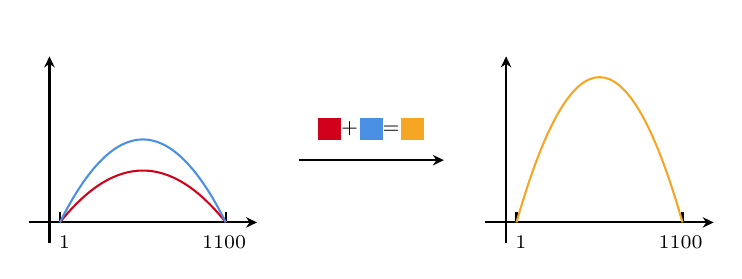
\begin{tikzpicture}[x=0.75pt,y=0.75pt,yscale=-1,xscale=1]
            %uncomment if require: \path (0,300); %set diagram left start at 0, and has height of 300

            %Straight Lines [id:da34248100016212457] 
            \draw    (170,90) -- (277,90) ;
            \draw [shift={(280,90)}, rotate = 180] [fill={rgb, 255:red, 0; green, 0; blue, 0 }  ][line width=0.08]  [draw opacity=0] (5.36,-2.57) -- (0,0) -- (5.36,2.57) -- (3.56,0) -- cycle    ;
            %Straight Lines [id:da8980030736411168] 
            \draw    (180,100) -- (180,13) ;
            \draw [shift={(180,10)}, rotate = 90] [fill={rgb, 255:red, 0; green, 0; blue, 0 }  ][line width=0.08]  [draw opacity=0] (5.36,-2.57) -- (0,0) -- (5.36,2.57) -- (3.56,0) -- cycle    ;
            %Straight Lines [id:da8756913546199198] 
            \draw [line width=0.75]    (185,85) -- (185,90) ;
            %Straight Lines [id:da1320233507901698] 
            \draw [line width=0.75]    (265,85) -- (265,90) ;
            %Shape: Parabola [id:dp8938018456449416] 
            \draw  [color={rgb, 255:red, 208; green, 2; blue, 27 }  ,draw opacity=1 ] (265,90) .. controls (238.33,56.67) and (211.67,56.67) .. (185,90) ;
            %Shape: Parabola [id:dp7154214398607968] 
            \draw  [color={rgb, 255:red, 74; green, 144; blue, 226 }  ,draw opacity=1 ] (265,90) .. controls (238.33,36.67) and (211.67,36.67) .. (185,90) ;
            %Straight Lines [id:da6661026753051024] 
            \draw    (390,90) -- (497,90) ;
            \draw [shift={(500,90)}, rotate = 180] [fill={rgb, 255:red, 0; green, 0; blue, 0 }  ][line width=0.08]  [draw opacity=0] (5.36,-2.57) -- (0,0) -- (5.36,2.57) -- (3.56,0) -- cycle    ;
            %Straight Lines [id:da5432422995538024] 
            \draw    (400,100) -- (400,13) ;
            \draw [shift={(400,10)}, rotate = 90] [fill={rgb, 255:red, 0; green, 0; blue, 0 }  ][line width=0.08]  [draw opacity=0] (5.36,-2.57) -- (0,0) -- (5.36,2.57) -- (3.56,0) -- cycle    ;
            %Straight Lines [id:da9027214096380924] 
            \draw [line width=0.75]    (405,85) -- (405,90) ;
            %Straight Lines [id:da6657825405781942] 
            \draw [line width=0.75]    (485,85) -- (485,90) ;
            %Shape: Parabola [id:dp0673950229164001] 
            \draw  [color={rgb, 255:red, 245; green, 166; blue, 35 }  ,draw opacity=1 ] (485,90) .. controls (458.33,-3.33) and (431.67,-3.33) .. (405,90) ;
            %Straight Lines [id:da6162418070851343] 
            \draw    (300,60) -- (367,60) ;
            \draw [shift={(370,60)}, rotate = 180] [fill={rgb, 255:red, 0; green, 0; blue, 0 }  ][line width=0.08]  [draw opacity=0] (5.36,-2.57) -- (0,0) -- (5.36,2.57) -- (3.56,0) -- cycle    ;
            %Shape: Rectangle [id:dp379274645803359] 
            \draw  [color={rgb, 255:red, 208; green, 2; blue, 27 }  ,draw opacity=1 ][fill={rgb, 255:red, 208; green, 2; blue, 27 }  ,fill opacity=1 ] (310,40) -- (320,40) -- (320,50) -- (310,50) -- cycle ;
            %Shape: Rectangle [id:dp8222817282747726] 
            \draw  [color={rgb, 255:red, 74; green, 144; blue, 226 }  ,draw opacity=1 ][fill={rgb, 255:red, 74; green, 144; blue, 226 }  ,fill opacity=1 ] (330,40) -- (340,40) -- (340,50) -- (330,50) -- cycle ;
            %Shape: Rectangle [id:dp557713999550064] 
            \draw  [color={rgb, 255:red, 245; green, 166; blue, 35 }  ,draw opacity=1 ][fill={rgb, 255:red, 245; green, 166; blue, 35 }  ,fill opacity=1 ] (350,40) -- (360,40) -- (360,50) -- (350,50) -- cycle ;

            % Text Node
            \draw (183,95) node [anchor=north west][inner sep=0.75pt]  [font=\scriptsize] [align=left] {$\displaystyle 1$};
            % Text Node
            \draw (252,95) node [anchor=north west][inner sep=0.75pt]  [font=\scriptsize] [align=left] {$\displaystyle 1100$};
            % Text Node
            \draw (403,95) node [anchor=north west][inner sep=0.75pt]  [font=\scriptsize] [align=left] {$\displaystyle 1$};
            % Text Node
            \draw (472,95) node [anchor=north west][inner sep=0.75pt]  [font=\scriptsize] [align=left] {$\displaystyle 1100$};
            % Text Node
            \draw (319,40) node [anchor=north west][inner sep=0.75pt]  [font=\scriptsize] [align=left] {$\displaystyle +$};
            % Text Node
            \draw (339,42) node [anchor=north west][inner sep=0.75pt]  [font=\scriptsize] [align=left] {=};
        \end{tikzpicture}
    \end{figure}

    Abgeschlossen bez. Multiplikation:

    \begin{figure}[h]
        \centering
        \tikzset{every picture/.style={line width=0.75pt}} %set default line width to 0.75pt        
        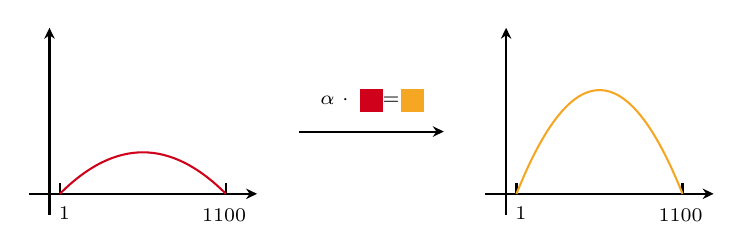
\begin{tikzpicture}[x=0.75pt,y=0.75pt,yscale=-1,xscale=1]
            %uncomment if require: \path (0,300); %set diagram left start at 0, and has height of 300

            %Straight Lines [id:da34248100016212457] 
            \draw    (170,90) -- (277,90) ;
            \draw [shift={(280,90)}, rotate = 180] [fill={rgb, 255:red, 0; green, 0; blue, 0 }  ][line width=0.08]  [draw opacity=0] (5.36,-2.57) -- (0,0) -- (5.36,2.57) -- (3.56,0) -- cycle    ;
            %Straight Lines [id:da8980030736411168] 
            \draw    (180,100) -- (180,13) ;
            \draw [shift={(180,10)}, rotate = 90] [fill={rgb, 255:red, 0; green, 0; blue, 0 }  ][line width=0.08]  [draw opacity=0] (5.36,-2.57) -- (0,0) -- (5.36,2.57) -- (3.56,0) -- cycle    ;
            %Straight Lines [id:da8756913546199198] 
            \draw [line width=0.75]    (185,85) -- (185,90) ;
            %Straight Lines [id:da1320233507901698] 
            \draw [line width=0.75]    (265,85) -- (265,90) ;
            %Shape: Parabola [id:dp8938018456449416] 
            \draw  [color={rgb, 255:red, 208; green, 2; blue, 27 }  ,draw opacity=1 ] (265,90) .. controls (238.33,63.33) and (211.67,63.33) .. (185,90) ;
            %Straight Lines [id:da6661026753051024] 
            \draw    (390,90) -- (497,90) ;
            \draw [shift={(500,90)}, rotate = 180] [fill={rgb, 255:red, 0; green, 0; blue, 0 }  ][line width=0.08]  [draw opacity=0] (5.36,-2.57) -- (0,0) -- (5.36,2.57) -- (3.56,0) -- cycle    ;
            %Straight Lines [id:da5432422995538024] 
            \draw    (400,100) -- (400,13) ;
            \draw [shift={(400,10)}, rotate = 90] [fill={rgb, 255:red, 0; green, 0; blue, 0 }  ][line width=0.08]  [draw opacity=0] (5.36,-2.57) -- (0,0) -- (5.36,2.57) -- (3.56,0) -- cycle    ;
            %Straight Lines [id:da9027214096380924] 
            \draw [line width=0.75]    (405,85) -- (405,90) ;
            %Straight Lines [id:da6657825405781942] 
            \draw [line width=0.75]    (485,85) -- (485,90) ;
            %Shape: Parabola [id:dp0673950229164001] 
            \draw  [color={rgb, 255:red, 245; green, 166; blue, 35 }  ,draw opacity=1 ] (485,90) .. controls (458.33,23.33) and (431.67,23.33) .. (405,90) ;
            %Straight Lines [id:da6162418070851343] 
            \draw    (300,60) -- (367,60) ;
            \draw [shift={(370,60)}, rotate = 180] [fill={rgb, 255:red, 0; green, 0; blue, 0 }  ][line width=0.08]  [draw opacity=0] (5.36,-2.57) -- (0,0) -- (5.36,2.57) -- (3.56,0) -- cycle    ;
            %Shape: Rectangle [id:dp379274645803359] 
            \draw  [color={rgb, 255:red, 208; green, 2; blue, 27 }  ,draw opacity=1 ][fill={rgb, 255:red, 208; green, 2; blue, 27 }  ,fill opacity=1 ] (330,40) -- (340,40) -- (340,50) -- (330,50) -- cycle ;
            %Shape: Rectangle [id:dp557713999550064] 
            \draw  [color={rgb, 255:red, 245; green, 166; blue, 35 }  ,draw opacity=1 ][fill={rgb, 255:red, 245; green, 166; blue, 35 }  ,fill opacity=1 ] (350,40) -- (360,40) -- (360,50) -- (350,50) -- cycle ;

            % Text Node
            \draw (183,95) node [anchor=north west][inner sep=0.75pt]  [font=\scriptsize] [align=left] {$\displaystyle 1$};
            % Text Node
            \draw (252,96) node [anchor=north west][inner sep=0.75pt]  [font=\scriptsize] [align=left] {$\displaystyle 1100$};
            % Text Node
            \draw (403,95) node [anchor=north west][inner sep=0.75pt]  [font=\scriptsize] [align=left] {$\displaystyle 1$};
            % Text Node
            \draw (472,96) node [anchor=north west][inner sep=0.75pt]  [font=\scriptsize] [align=left] {$\displaystyle 1100$};
            % Text Node
            \draw (339,42) node [anchor=north west][inner sep=0.75pt]  [font=\scriptsize] [align=left] {=};
            % Text Node
            \draw (309,41) node [anchor=north west][inner sep=0.75pt]  [font=\scriptsize] [align=left] {$\displaystyle \alpha \ \cdotp $};
        \end{tikzpicture}
    \end{figure}

    \( \{p \in \mathcal{P}_3\: |\: p(1) = 0 \) und  \( p(1100)=0\} \subset \mathcal{P}_3 \) ist ein Unterraum.

    \vspace{1\baselineskip}

    \textbf{d)}

    Enthält den Nullvektor: \( |0| + |0| = |0| \)

    \vspace{0.5\baselineskip}

    Abgeschlossen bez. Addition:

    \begin{equation*}
        \begin{pmatrix}
            1 \\ 0 \\ 1
        \end{pmatrix} + \begin{pmatrix}
            0 \\ -1 \\ -1
        \end{pmatrix} = \begin{pmatrix}
            1 \\ -1 \\ 0
        \end{pmatrix} \quad \Rightarrow \quad |1| + |-1| = |2| \neq |0|
    \end{equation*}

    Nicht abgeschlossen bez. Addition, also kein Unterraum.

\end{solution}

\newpage

\subsubsection{} %Adi PVK Tag 2

Betrachten Sie den Vektorraum \( \mathcal{P}_3 \) der reellen Polynome vom Grad \( \leq \) 3 mit der Basis \( \mathcal{B} = \{x^3+1,x^2+x-2,2x+1,x+2\} \).

\begin{enumerate}[label=\alph*)]
    \item Welches Polynom in \( \mathcal{P}_3 \) hat die Koordinaten \( (2,1,-1,3)^\top \) bezüglich \( \mathcal{B} \)?
    \item Sei \( p(x):=x^3+x^2+x+1 \). Bestimmen Sie die Koordinaten von \( p(x) \) bezüglich \( \mathcal{B} \).
\end{enumerate}

\vspace{1\baselineskip}

\begin{solution}    

    \vspace{1\baselineskip}

    \leftskip=2em

    \textbf{a)}

    \begin{equation*}
        \begin{aligned}
            p(x) &= 2(x^3+1) + 1(x^2+x-2) - 1(2x+1) + 3(x+2) \\
            &= 2x^3 + 2 + x^2 + x - 2 - 2x - 1 + 3x + 6 \\            
            &= 2x^3 + x^2 + 2x + 5.
        \end{aligned}
    \end{equation*}

    \textbf{b)}

    \begin{equation*}
        \begin{gmatrix}[L]
            1 & 0 & 0 & 0 \\
            0 & 1 & 0 & 0 \\
            0 & 1 & 2 & 1 \\
            1 & -2 & 1 & 2
        \end{gmatrix} \hspace{-0.75em} \begin{gmatrix}[R]
            1 \\ 1 \\ 1 \\ 1
            \rowops
                \add[-1]{0}{3}
        \end{gmatrix} \rightarrow \; \begin{gmatrix}[L]
            1 & 0 & 0 & 0 \\
            0 & 1 & 0 & 0 \\
            0 & 1 & 2 & 1 \\
            0 & -2 & 1 & 2
        \end{gmatrix} \hspace{-0.75em} \begin{gmatrix}[R]
            1 \\ 1 \\ 1 \\ 0
            \rowops
                \add[-1]{1}{2}
                \add[2]{1}{3}
        \end{gmatrix} \hspace{-0.75em} \rightarrow \; \begin{gmatrix}[L]
            1 & 0 & 0 & 0 \\
            0 & 1 & 0 & 0 \\
            0 & 0 & 2 & 1 \\
            0 & 0 & 1 & 2
        \end{gmatrix} \hspace{-0.75em} \begin{gmatrix}[R]
            1 \\ 1 \\ 0 \\ 2
            \rowops
                \swap{2}{3}
            \end{gmatrix} 
    \end{equation*}

    \vspace{0.5\baselineskip}

    \begin{equation*}
        \rightarrow \;
        \begin{gmatrix}[L]
            1 & 0 & 0 & 0 \\
            0 & 1 & 0 & 0 \\
            0 & 0 & 1 & 2 \\
            0 & 0 & 2 & 1
        \end{gmatrix} \hspace{-0.75em} \begin{gmatrix}[R]
            1 \\ 1 \\ 2 \\ 0
            \rowops
                \add[-2]{2}{3}
        \end{gmatrix} \rightarrow \; \begin{gmatrix}[L]
            1 & 0 & 0 & 0 \\
            0 & 1 & 0 & 0 \\
            0 & 0 & 1 & 2 \\
            0 & 0 & 0 & -3
        \end{gmatrix} \hspace{-0.75em} \begin{gmatrix}[R]
            1 \\ 1 \\ 2 \\ -4
        \end{gmatrix} \rightarrow \quad \begin{aligned}
            x_4 &= \frac{4}{3} \\
            x_3 &= - \frac{2}{3} \\
            x_2 &= 1 \\
            x_1 &= 1
        \end{aligned}
    \end{equation*}

    Die Koordinaten von \( p(x) \) bezüglich \( \mathcal{B} \) sind also

    \begin{equation*}
        [p(x)]_{\mathcal{B}} = \begin{pmatrix}
            1 \\ 1 \\ -\frac{2}{3} \\ \frac{4}{3}
        \end{pmatrix}.
    \end{equation*}

\end{solution}

\newpage

\subsubsection{} %Prüfung S12

Sei \( V \) der von den Funktionen \( \{1,x,x^2,e^x\} \) aufgespannte Vektorraum mit dem Unterraum \( U:=\{1,x,x^2\} \). Für zwei Funktionen \( f,g \in V \) sei das folgende Skalarprodukt definiert:

\begin{equation*}
    \langle f,g \rangle := f(0)g(0)+f'(0)g'(0)+f''(0)g''(0)+f'''(0)g'''(0).
\end{equation*}

\begin{enumerate}[label=\alph*)]
    \item Wie lautet die Norm von \( f \in V \) bezüglich des gegebenen Skalarprodukts?
    \item Bestimmen Sie eine Orthonormalbasis in \( U \) bezüglich des gegebenen Skalarprodukts.
    \item Verifizieren Sie, dass \( \langle . \:,. \rangle \) tatsächlich ein Skalarprodukt ist.
\end{enumerate}

\vspace{1\baselineskip}

\begin{solution}    

    \vspace{1\baselineskip}

    \leftskip=2em

    \textbf{a)} \( \qquad ||f|| = \sqrt{f(0)^2 + f'(0)^2 + f''(0)^2 + f'''(0)^2} \)

    \vspace{1.5\baselineskip}

    \textbf{b)} Gram-Schmidt: \( b_1 = 1, \ b_2 = x, \ b_3 = x^2 \)

    \begin{equation*}
        \begin{aligned}
            \rightarrow \ e_1 &= \frac{1}{||1||} \qquad \qquad \rightarrow e_2' = b_2 - \underbrace{\langle b_2,e_1 \rangle}_{=0} e_1 = x \\
            & \hspace{3.65cm} e_2 = \frac{e_2'}{||e_2'||} = x \\[1.75em]
            \rightarrow e_3' &= b_3 - \underbrace{\langle b_3,e_2 \rangle}_{=0} e_2 - \underbrace{\langle b_3,e_1 \rangle}_{=0} e_1 = x^2 \\
            \qquad e_3 &= \frac{e_3'}{||e_3'||} = \frac{x^2}{2} \hspace{5cm} \mathcal{B} = \left\{ 1, x, \frac{x^2}{2} \right\}
        \end{aligned}
    \end{equation*}

    \vspace{1\baselineskip}

    \textbf{c)} \( \quad x, y, z \in V \)
    
    \begin{equation*}
        \begin{aligned}
            \textcolor{red}{\langle x, y+z \rangle} &= x(0)[y(0)+z(0)] + x'(0)[y'(0)+z'(0)] + x''(0)[y''(0)+z''(0)] \\ 
            & \quad + x'''(0)[y'''(0)+z'''(0)] \\
            &= x(0)y(0) + x(0)z(0) + x'(0)y'(0) + x'(0)z'(0) + x''(0)y''(0) \\
            & \quad + x''(0)z''(0) + x'''(0)y'''(0) + x'''(0)z'''(0) = \textcolor{red}{\langle x,y \rangle + \langle x,z \rangle}. \\[0.5em]
            \textcolor{red}{\langle x, \alpha y \rangle} &= x(0)(\alpha y(0)) + x'(0)(\alpha y'(0)) + x''(0)(\alpha y''(0)) + x'''(0)(\alpha y'''(0)) \\
            &= \alpha \left[ x(0)y(0) + x'(0)y'(0) + x''(0)y''(0) + x'''(0)y'''(0) \right] = \textcolor{red}{\alpha \langle x,y \rangle}. \\[0.5em]
            \textcolor{red}{\langle x, y \rangle} &= x(0)y(0) + x'(0)y'(0) + x''(0)y''(0) + x'''(0)y'''(0) = \textcolor{red}{\langle y, x \rangle}. \\[0.5em]
            \textcolor{red}{\langle x, x \rangle} &= x(0)^2 + x'(0)^2 + x''(0)^2 + x'''(0)^2 \ \textcolor{red}{\geq 0}. \\[0.5em]
            \textcolor{red}{\langle f, f \rangle} &= 0 \; \Leftrightarrow \; \textcolor{red}{f \equiv 0}, \ e^x-\text{Term sonst nie Null}. 
        \end{aligned}
    \end{equation*}


\end{solution}

\newpage

\subsubsection{} %Zardini S.70

Sei folgendes Skalarprodukt auf \( \mathcal{P}_4 \) gegeben

\begin{equation*}
    \langle p,q \rangle = \int_{0}^{1} p(x)q(x) \,dx.
\end{equation*}

Finden Sie eine Orthonormalbasis für den Vektorraum span\( \{1,3x^4\} \). 

\vspace{1\baselineskip}

\begin{solution}    

    \vspace{1\baselineskip}

    \leftskip=2em

    Gram-Schmidt: \( b_1 = 1, \ b_2 = 3x^4 \)

    \begin{equation*}
        \begin{aligned}
            \rightarrow e_1 &= \frac{b_1}{||b_1||} = 1 \\[2em]
            \rightarrow e_2' &= b_2 - \underbrace{\langle b_2,e_1 \rangle} e_1 \\
            & \hspace{1.65cm} \int_{0}^{1} 3x^4 dx = \frac{3}{5} \\[0.5em]
            e_2' &= 3x^4 - \frac{3}{5} \\[1.5em]
            e_2 &= \frac{e_2'}{||e_2'||} \\
            & \hspace{0.6cm} ||e_2'|| = \sqrt{\int_{0}^{1} (3x^4 - \frac{3}{5})^2 dx} = \frac{4}{5} \\[0.5em]
            e_2 &= \frac{5}{4} (3x^4 - \frac{3}{5}) = \frac{3}{4}(5x^4 - 1)
        \end{aligned}
    \end{equation*}

    \vspace{1\baselineskip}

    Eine Orthonormalbasis ist dann gegeben durch

    \begin{equation*}
        \mathcal{B} = \left\{ 1, \frac{3}{4}(5x^4 - 1) \right\}.
    \end{equation*}

\end{solution}
